%%%%%%%%%%%%%%%%%%%%%%%%%%%%%%%%%%%%%%%%%%%%%%%%%%%%%%%%%%%
% EPFL report package, main thesis file
% Goal: provide formatting for theses and project reports
% Author: Mathias Payer <mathias.payer@epfl.ch>
%
% This work may be distributed and/or modified under the
% conditions of the LaTeX Project Public License, either version 1.3
% of this license or (at your option) any later version.
% The latest version of this license is in
%   http://www.latex-project.org/lppl.txt
%
%%%%%%%%%%%%%%%%%%%%%%%%%%%%%%%%%%%%%%%%%%%%%%%%%%%%%%%%%%%
\documentclass[a4paper,11pt,oneside]{report}
% Options: MScThesis, BScThesis, MScProject, BScProject
\usepackage[MScThesis,lablogo]{EPFLreport}
\usepackage{xspace}
\usepackage{listings}

\lstset{ 
  basicstyle=\footnotesize,        % the size of the fonts that are used for the code
  frame=single,	                   % adds a frame around the code
  language=C++,                    % the language of the code
}

\title{Recovering type information from compiled binaries\\to aid in instrumentation}
\author{Louis Merlin}
\supervisor{Antony Vennard}
\adviser{Prof. Dr. sc. ETH Mathias Payer}
%\coadviser{Second Adviser}
\expert{Damian Pfammatter}

\newcommand{\sysname}{FooSystem\xspace}

\setlength{\parindent}{0cm}

\begin{document}
\maketitle
\makededication
\makeacks

\begin{abstract}
The abstract serves as an executive summary of your project.
Your abstract should cover at least the following topics, 1-2 sentences for
each: what area you are in, the problem you focus on, why existing work is
insufficient, what the high-level intuition of your work is, maybe a neat
design or implementation decision, and key results of your evaluation.
\end{abstract}

% \begin{frenchabstract}
% For a doctoral thesis, you have to provide a French translation of the
% English abstract. For other projects this is optional.
% \end{frenchabstract}

\maketoc

%%%%%%%%%%%%%%%%%%%%%%
\chapter{Introduction}
%%%%%%%%%%%%%%%%%%%%%%

% The introduction is a longer writeup that gently eases the reader into your
% thesis~\cite{dinesh20oakland}. Use the first paragraph to discuss the setting.
% In the second paragraph you can introduce the main challenge that you see.
% The third paragraph lists why related work is insufficient.
% The fourth and fifth paragraphs discuss your approach and why it is needed.
% The sixth paragraph will introduce your thesis statement. Think how you can
% distill the essence of your thesis into a single sentence.
% The seventh paragraph will highlight some of your results
% The eights paragraph discusses your core contribution.

% This section is usually 3-5 pages.


% Setting: compiled binaries; RetroWrite; [need for a compatible exchange format => DWARF;] closed-source C++ binaries in the wild (android?).

Work on C++ began in 1979, as a "C with classes"~\cite{cwithclasses}.
Since then, the language has grown in popularity, and even surpassed C itself~\cite{stackoverflowpopularity}.
Examples of well-known C++ projects include the zoom~\cite{zoom} conferencing software, the gold linker~\cite{gold} or [TODO: find another "well-known" example].
Nevertheless, reverse-engineering efforts have been focused towards C binaries, because analysis methods found this way will often work on C++ binaries too.


% Main challenge:
% C++-specific ELF sections are not as well documented as they could be (?);
% Debuggers do not work as well as they should on non-C binaries;

This has meant reverse engineering tools like ghidra~\cite{ghidra}, IDA Pro~\cite{ida} or Binary Ninja~\cite{binja} have treated non-C binaries as second-class citizen.
These tools will often show C++ specific features as passing comments, failing to show the real implications of a try/catch block or a polymorphic class.

% Ghidra/IDA will show as pseudo-C code, but not C++
%  see throw/catch or RTTI
% C++ is quite a compilicated language.
% C's abstractions work very well in assembler, but C++ adds a whole layer of complexity.
% When translated to assembly, a lot of information is lost.

The blame can mostly be put on the complexity of C++ when compared to C.
Whereas C translates quite naturally to assembly, abstractions specific to C++ require more work and complexity to be translated to asm.
This also leads to important information being lost from C++ source code to binary, but also certain information remaining.


% Related work:
% RetroWrite only does C;
% debugging tools don't have nice support for C++ features;
% DWARF will be explored more and more in the coming years;

The recent RetroWrite~\cite{dinesh20oakland} project by the HexHive lab is a static rewriting tool for x86\_64 position-independent binaries.
It enables the instrumentation of projects when we do not have access to the source code.
This can include a legacy project, a closed-source product or even malware.

% Does anything else try to do retrowriting C++ ?
% Does anything else try to extract classes ? (Marx / plugins)


% Our approach:
% Tool for static analysis of C++ binaries, to recover classes and display them in a helpful way;
% Fixing RetroWrite to support C++ binaries;

In this thesis we would like to present the \textbf{dis-cover}~\cite{discovergithub} static analysis tool,
as well as improvements made to RetroWrite to support C++ binaries.


% Why it is needed:
% Non-obtrusive way of adding C++ support in debugging tools;
% Nobody (?) (as far as we know / to the best of our knowledge) has been able to rewrite C++ binaries before, this could lead to very interesting discoveries;

The dis-cover tool is able to extract information from a C++ binary, and re-inject it as debug information using the DWARF format into the binary.
This enables other debugging tools to see and display this information.


% Highlight results:
% 53\% of packages on Debian that use C++ have extracteable classes;
% [whatever we are able to do with C++ and RetroWrite];


% It's a first symbolic representation of C++ code that can be recompiled


% Core contribution:
% dis-cover as an open-source tool;
% [whatever we are able to add to RetroWrite];
% Also the documentation of the process.

[IF WE SUCCEEDED]
In this thesis we would like to show how we brought C++ support to RetroWrite, and what research opportunities this will create.

[IF WE FAILED]
In this thesis we will detail how we tried to bring C++ support to RetroWrite, and what remains to be done for the implementation to work.


%%%%%%%%%%%%%%%%%%%%
\chapter{Background}
%%%%%%%%%%%%%%%%%%%%

% The background section introduces the necessary background to understand your
% work. This is not necessarily related work but technologies and dependencies
% that must be resolved to understand your design and implementation.

% This section is usually 3-5 pages.

\section{C++ and polymorphism}

% C++ polymorphism (what, how, but also research like Marx) (+ exceptions) 
% also talk about how compilers will optimize this out in certain situtations
The C++ programming language implements polymorphism.
This feature enables complex code logic that can comply with external business logic for example.
Polymorphic classes are defined by having at least one virtual method, which is inheritable and overridable.
With this polymorphism comes type conversion, and more interestingly for us the \textbf{dynamic\_cast}~\cite{dynamiccast} expression.
Dynamic casting is a safe kind of type conversion.
It only will successfully cast if the value is of the referenced type or a base type of that type.
In order to achieve that, the system must have some kind of information about the object's data type at run time.

This is where Run-Time Type Information (\textbf{RTTI}) comes into the picture.
The system will use this RTTI to infer type inheritance for dynamic casting.
We will now go into implementation details of RTTIs and VTables, which point to them.

To make RTTIs appear in your C++ binary, you will to define classes that inherit from each other, as well as at least one virtual method in one of these classes.
\autoref{classes} shows an example of such classes.

\begin{figure}[h]
\begin{lstlisting}
class Animal {
public:
  virtual void speak() {}
};

class Dog {
public:
  virtual void speak() { cout << "Woof" << endl; }
}
\end{lstlisting}
\caption{Polymorphic classes in C++}
\label{classes}

\end{figure}

For RTTIs to appear in your C++ binary, you will also need to instantiate these classes, and have some run time logic to make the binary non-deterministic [this not the right word I think, I mean to say that the binary depends on some input for its class-instantiating logic].
For example, a conditional dynamic cast between the two classes we defined in \autoref{classes}.
If you do not do these things, the class logic will be abstracted away by the compiler for optimization reasons.

\begin{figure}[h]

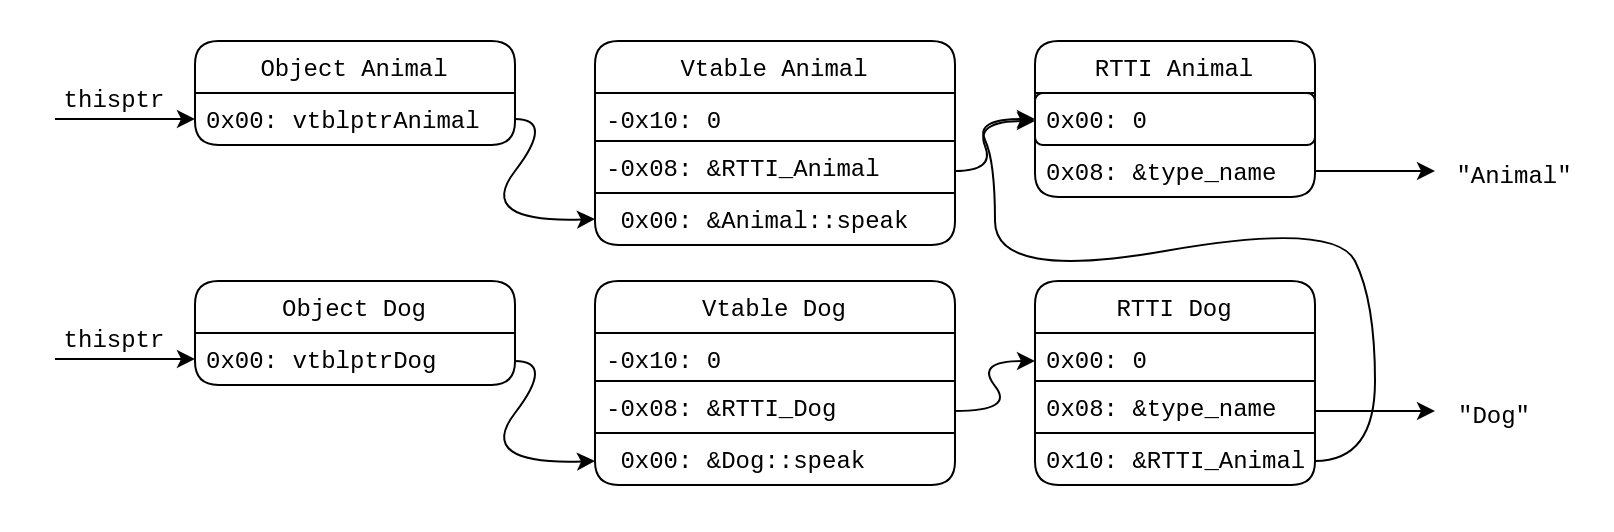
\includegraphics[width=16cm]{RTTI_graph.png}
\caption{Overview of an example of VTables and RTTI in memory}
\label{rttigraph}

\end{figure}

The structure of VTables and RTTIs is detailed in \autoref{rttigraph}.
All of this is defined in the Itanium C++ ABI~\cite{cppabi}.
An instance of a virtual class Animal will contain the \textbf{vtblptrAnimal}, a pointer to the virtual table (\textbf{VTable}) for the Animal class.
This VTable will contain pointers to the virtual methods of the class, which are inherited and thus do not have to be duplicated for each class, they are simply pointed to.
The first value preceding the VTable is a pointer to the RTTI of the class. The process finds out the class inheritance of a class instance by following this pointer.

The RTTI itself is composed of an offset (used for complex class inheritance structures) as well as a pointer to the type name (this type name is not removed by simple stripping of the binary, like with \textbf{objdcopy --strip-all}).
This name is mangled using C++ mangling, and can trivially be de-mangled. This name is what we use to uniquely identify a class in a project (and make sure we have no duplicates).
The next values of the RTTI are pointers to the RTTIs of the parent classes. See \autoref{rttigraph} for an example, with the Dog RTTI containing a pointer to the Animal RTTI.

\section{DWARF debugging standard}

% DWARF DIEs
\textbf{DWARF} is the debugging standard used widely in conjunction with executable ELF files.
It is often included in these ELF files in the \textbf{.debug\_info} section (and other related sections).
This debug information is made up of Debugging Information Entries (\textbf{DIEs}).
These entries can contain information about variable names, method definitions, the compilation process, or more importantly for us, class names and class inheritance.

% ELF sections

\section{RetroWrite}

% How RetroWrite works


%%%%%%%%%%%%%%%%
\chapter{Design}
%%%%%%%%%%%%%%%%

Introduce and discuss the design decisions that you made during this project.
Highlight why individual decisions are important and/or necessary. Discuss
how the design fits together.

This section is usually 5-10 pages.

% Design => Decisions
% We decided not to reproduce Marx's work
% First attempt : recover classes from RTTI
% Future work : could take approaches like Marx and re-feed it like us
Class recovery from compiled C++ binaries has been done multiple ways before:
there are plugins for popular debugging tools, like ida\_gcc\_rtti~\cite{idagccrtti} for IDA Pro,
or Ghidra-Cpp-Class-Analyzer~\cite{ghidracppclassanalyzer} for Ghidra;
there are academic projects such as MARX~\cite{marx} that rely on heuristics around VTables to find classes and inheritance information.
The MARX project can recover classes when no RTTI is present (in the Chrome project for example, where the \textbf{fno-rrti} compilation flag is used), but not with 100\% accuracy.

% VTable => RTTI
%   mention class data (Debian analysis)
For this project we decided to focus on RTTIs which, as mentioned in the Background chapter, are available for a class hierarchy tree when there is at least one virtual method implemented by one of the classes.
We decided to test if RTTIs occurred often in the wild : we proceed to download every Debian package that listed C++ as a dependency (get the list with \textbf{apt-cache rdepends libgcc1} on a Debian machine).
Out of around 80'000 packages, 5827 of them list C++ as a dependency.
Out of those, we extracted classes from 3194 (54\%).
We will share more details about this experiment in the Evaluation chapter.

% Also: exceptions (we felt this needed to be handled)
We also considered extracting information about exceptions, which is another big feature that differentiates C++ from C.
We decided not to focus on this feature, as it did not seem to bring as much to the project considering the evaluated development time.
We did have to study and work with exceptions and exception handling frames for the augmentation of RetroWrite (see the end of the Implementation chapter).

% Why do we want DWARF data ?
%   We want to make the info available to reversing tools
%   => input from Dr. Sergey Bratus
%        He would like to see DWARF used as a lingua franca for debugging
% Also, exception's try/catch blocks & exception types
% but dwarf is limited for this (=> future work)
Next comes the question : what should we do with all of this information ? What would be the most useful format to output the data in ?
This is where DWARF~\cite{dwarf} comes in the picture. DWARF is the debugging standard for programs.
It is mostly used by developers trying to understand where their implementation fails,
and by reverse engineers to get a better understanding of how a program was conceived (although DWARF information is usually stripped from proprietary software).
This kind of debug data is mostly found in C and C++ projects. % Should I add another language ?
By having DWARF data as an output, the information would become readable by most modern reversing tools.

There is a current push for DWARF to become the lingua franca for reverse engineering tools, lead by researchers like Dr. Sergey Bratus~\cite{bratus} from DARPA.
He has published a paper in 2011 where he was able to exploit certain features of DWARF to control program execution : Exploiting the hard-working DWARF~\cite{hardworkingdwarf}.

% Injecting debug section & symbols
With dis-cover, we are able to inject information in the debug and symbol sections of the binary, creating a new ELF file with all of this useful info included.
We will go more into the implementation details in the next chapter.

% RetroWrite structure
%  x86_64 userspace and kernel, and arm_64
%  We've decided to focus on the x86_64 userspace
%    Most widely used target
%    Kernel drivers are mostly written in C
% We still want to keep the deterministic ability of retrowrite
Another focus of this project was the augmentation of RetroWrite for C++ capabilities.
Today, RetroWrite supports the reversing of x86\_64 position-independent binaries.
There was also work to augment RetroWrite to support kernel code~\cite{rwkernel} and arm\_64~\cite{rwarm}.
We aimed to add C++ capabilities for x86\_64 binaries only, as it seems like the biggest target.

Another potential use of the class information is to implement defenses around type confusion, working with the findings from the HexType~\cite{hextype} paper.
We decided not to focus on this for our project, as it would have been out of the scope of a 6-months master thesis.

One of the defining properties of RetroWrite is that it does not use heuristics (and thus does not have probabilistic features and failures).
Dis-cover has the same no-heuristics property, and thus could be used by the RetroWrite project without breaking the property.


%%%%%%%%%%%%%%%%%%%%%%%%
\chapter{Implementation}
%%%%%%%%%%%%%%%%%%%%%%%%

% The implementation covers some of the implementation details of your project.
% This is not intended to be a low level description of every line of code that
% you wrote but covers the implementation aspects of the projects.

% This section is usually 3-5 pages.

% Python script (because RetroWrite; and good tools) (1 sentence)
We decided to write a python module for this project, as the python ecosystem has great reverse engineering packages, and because the other projects from the HexHive lab are usually python modules.

\section{Finding RTTIs}

% RTTI and VTable
The first thing dis-cover does is find ELF sections where the VTables and RTTIs could be hiding.
This is usually \textbf{.rodata} (read-only data), but could sometimes also be related sections like \textbf{.data.rel.ro}, \textbf{.data.rel.ro.local}, or \textbf{.rdata}.
[TODO see if we can just look in .rodata]
As per the Itanium C++ ABI, the base VTable of a class will contain an "offset-to-top", which will be 0 in the primary base virtual table's case, followed by a pointer to an RTTI.
We simply have to pattern-match for zeroes directly followed by a pointer to another part of the read-only data sections, and we have a potential RTTI pointer.

To check whether we have found an RTTI, we assert that the next value is a pointer to a string located in a read-only data section.
If it is, we can extract it, demangle it, and we have a class and a name.
The next values in the RTTI are pointers to the RTTIs the class inherits from.
We can go through them and parse them if we have not already, to add this inheritance information to the original class.

This algorithm is $O(n)$, as adding a class only adds one more value to parse.

\section{Creating DWARF data}

% Creating DIEs
Next, we want to add that information to the debug sections of a new ELF file.

% DIE Bytecode
In order to write DWARF data, the first step is defining the types we will be using, and their fields.
This is done by writing bytes in the \textbf{.debug\_abbrev} section.
For example, we create an abbrev of type \textbf{class\_type}, which has a \textbf{name}, and can have sub-field (children).
Then, we create the abbrev of type \textbf{inheritance}, which has a \textbf{type} (a reference to the parent type).

We can then populate the \textbf{.debug\_info} with classes and their inheritance data.
DWARF data takes the form of a tree of values. We have to create a \textbf{compile\_unit} value at the root, and then the branches will be \textbf{class\_type}s.
These \textbf{class\_type}s will themselves have as children \textbf{inheritance} values if the class inherits from another class.

TODO Add a figure with the output from dwarfdump for a simple example.

% unwind tables etc
% what it does and does not do

% eu-unstrip etc

% RetroWrite implementation details
% Refer to the other thesis

%%%%%%%%%%%%%%%%%%%%
\chapter{Evaluation}
%%%%%%%%%%%%%%%%%%%%

In the evaluation you convince the reader that your design works as intended.
Describe the evaluation setup, the designed experiments, and how the
experiments showcase the individual points you want to prove.

This section is usually 5-10 pages.

% Small examples

% Big applications examples

% Debian test
As we have shown before, out of the 5827 debian packages that list C++ as a dependency, we were able to extract classes from 3194 (54\%).
The total number of classes we found is 960'188, with 39\% of them unique across all packages (unique name in unique tree).

% RetroWrite test


%%%%%%%%%%%%%%%%%%%%%%
\chapter{Related Work}
%%%%%%%%%%%%%%%%%%%%%%

The related work section covers closely related work. Here you can highlight
the related work, how it solved the problem, and why it solved a different
problem. Do not play down the importance of related work, all of these
systems have been published and evaluated! Say what is different and how
you overcome some of the weaknesses of related work by discussing the 
trade-offs. Stay positive!

This section is usually 3-5 pages.

% Marx


%%%%%%%%%%%%%%%%%%%%
\chapter{Conclusion}
%%%%%%%%%%%%%%%%%%%%

In the conclusion you repeat the main result and finalize the discussion of
your project. Mention the core results and why as well as how your system
advances the status quo.

\cleardoublepage
\phantomsection
\addcontentsline{toc}{chapter}{Bibliography}
\printbibliography

% Appendices are optional
% \appendix
% %%%%%%%%%%%%%%%%%%%%%%%%%%%%%%%%%%%%%%
% \chapter{How to make a transmogrifier}
% %%%%%%%%%%%%%%%%%%%%%%%%%%%%%%%%%%%%%%
%
% In case you ever need an (optional) appendix.
%
% You need the following items:
% \begin{itemize}
% \item A box
% \item Crayons
% \item A self-aware 5-year old
% \end{itemize}

\end{document}
